\chapter{Pattern Matching}

\section{Hubungan antara Elixir, Erlang, dan BEAM}

Diagram berikut menggambarkan hubungan antara Elixir, Erlang, dan BEAM:

\begin{center}
	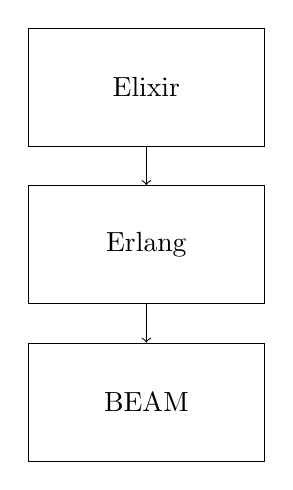
\begin{tikzpicture}[node distance=2cm]
		\node (elixir) [rectangle, draw, text centered, minimum height=1.5cm, minimum width=3cm] {Elixir};
		\node (erlang) [rectangle, draw, below of=elixir, text centered, minimum height=1.5cm, minimum width=3cm] {Erlang};
		\node (beam) [rectangle, draw, below of=erlang, text centered, minimum height=1.5cm, minimum width=3cm] {BEAM};
		
		\draw[->] (elixir) -- (erlang);
		\draw[->] (erlang) -- (beam);
	\end{tikzpicture}
\end{center}

\subsection{Elixir}

Elixir adalah bahasa pemrograman yang modern dan dinamis, dikembangkan untuk memenuhi kebutuhan aplikasi terdistribusi yang skalabel dan fault-tolerant. Meskipun Elixir memiliki sintaks yang berbeda dan modern, ia bergantung sepenuhnya pada ekosistem Erlang untuk menjalankan aplikasinya.

\subsection{Erlang}

Erlang adalah bahasa pemrograman yang mendasari Elixir. Ketika kode Elixir dikompilasi, ia diubah menjadi bytecode Erlang. Ini memungkinkan Elixir untuk memanfaatkan seluruh ekosistem Erlang, termasuk pustaka, alat, dan framework yang sudah ada. Dengan kata lain, Elixir adalah lapisan di atas Erlang yang menyediakan sintaks dan fitur tambahan sambil tetap menggunakan fondasi yang kuat dari Erlang.

\subsection{BEAM}

BEAM (Bogdan/Björn's Erlang Abstract Machine) adalah mesin virtual yang menjalankan bytecode Erlang, termasuk kode yang ditulis dalam Elixir. BEAM dirancang untuk mendukung concurrency, fault-tolerance, dan distribusi yang dibutuhkan oleh aplikasi Elixir dan Erlang. BEAM adalah komponen inti yang membuat Elixir dan Erlang mampu menangani jutaan proses secara efisien.

\subsection{Hubungan dalam Diagram}

Diagram di atas menunjukkan bagaimana Elixir bergantung pada Erlang dan akhirnya dijalankan di atas BEAM. Ketika seorang pengembang menulis kode dalam Elixir, kode tersebut pertama-tama diterjemahkan menjadi bytecode Erlang. Selanjutnya, bytecode tersebut dijalankan oleh BEAM, yang mengelola eksekusi program secara efisien. Ini berarti meskipun Elixir dan Erlang adalah bahasa yang berbeda, mereka berbagi mesin runtime yang sama, yaitu BEAM, yang membuat mereka sangat kompatibel dan interoperabel.

\section{Pattern Matching di Elixir}

Pattern matching adalah salah satu fitur paling kuat dan fundamental dalam bahasa pemrograman Elixir. Fitur ini memungkinkan pengembang untuk mencocokkan struktur data dan mengekstrak nilai-nilai dari struktur tersebut secara deklaratif. Tidak seperti bahasa pemrograman imperatif di mana variabel diinisialisasi dengan nilai, dalam Elixir, pattern matching berfungsi sebagai alat untuk membandingkan dan mengurai data.

\subsection{Dasar-Dasar Pattern Matching}

Pada dasarnya, pattern matching menggunakan operator \texttt{=} untuk mencocokkan sisi kiri dan sisi kanan dari ekspresi. Jika keduanya cocok, maka Elixir akan mengikat nilai dari sisi kanan ke variabel di sisi kiri.

\begin{lstlisting}[language=Elixir]
	iex> x = 1
	1
	
	iex> 1 = x
	1
\end{lstlisting}

Dalam contoh di atas, nilai 1 di sisi kanan diikat ke variabel \texttt{x}. Karena sisi kiri dan kanan dari ekspresi \texttt{1 = x} cocok, Elixir hanya mengembalikan \texttt{1}.

\subsection{Pattern Matching dengan Tuple}

Pattern matching sangat berguna ketika bekerja dengan struktur data yang lebih kompleks seperti tuple.

\begin{lstlisting}[language=Elixir]
	iex> {a, b, c} = {1, 2, 3}
	{1, 2, 3}
	
	iex> a
	1
	
	iex> b
	2
	
	iex> c
	3
\end{lstlisting}

Dalam contoh di atas, tuple \texttt{\{1, 2, 3\}} dicocokkan dengan pola \texttt{\{a, b, c\}}, sehingga nilai-nilai di dalam tuple diikat ke variabel \texttt{a}, \texttt{b}, dan \texttt{c}.

\subsection{Pattern Matching dengan List}

Pattern matching juga dapat digunakan dengan list, termasuk penggunaan \texttt{head} dan \texttt{tail} untuk mencocokkan bagian pertama dari list dan sisa elemennya.

\begin{lstlisting}[language=Elixir]
	iex> [head | tail] = [1, 2, 3]
	[1, 2, 3]
	
	iex> head
	1
	
	iex> tail
	[2, 3]
\end{lstlisting}

Di sini, \texttt{head} mendapatkan nilai pertama dari list, sedangkan \texttt{tail} mendapatkan list yang tersisa.

\subsection{Menggunakan Pattern Matching dalam Fungsi}

Pattern matching dapat digunakan dalam definisi fungsi untuk membuat kode yang lebih bersih dan mudah dibaca.

\begin{lstlisting}[language=Elixir]
	defmodule Example do
	def greet({first_name, last_name}) do
	"Hello, #{first_name} #{last_name}!"
	end
	end
	
	iex> Example.greet({"John", "Doe"})
	"Hello, John Doe!"
\end{lstlisting}

Pada contoh ini, fungsi \texttt{greet/1} menerima tuple yang terdiri dari \texttt{first\_name} dan \texttt{last\_name}. Nilai-nilai ini langsung dicocokkan dengan pola yang didefinisikan dalam parameter fungsi.

\subsection{Pattern Matching dengan Pengkondisian}

Berikut adalah contoh penggunaan \texttt{case} dengan pattern matching di dalam modul dan fungsi Elixir:

\begin{lstlisting}[language=Elixir]
defmodule Example do
	def match_pattern(tuple) do
		case tuple do
		{1, x, 3} -> IO.puts("x adalah #{x}")
		_ -> IO.puts("Tidak ada kecocokan")
		end
	end
end

# Pemanggilan fungsi
Example.match_pattern({1, 2, 3})
\end{lstlisting}

Pada contoh ini, modul \texttt{Example} berisi fungsi \texttt{match\_pattern/1} yang melakukan pattern matching terhadap tuple yang diterima sebagai argumen. Jika tuple sesuai dengan pola \texttt{\{1, x, 3\}}, maka nilai \texttt{x} dicetak. Jika tidak, pesan \texttt{"Tidak ada kecocokan"} akan ditampilkan.

\begin{verbatim}
	x adalah 2
\end{verbatim}


Pattern matching di Elixir memungkinkan pemrograman yang lebih deklaratif dan ekspresif. Dengan kemampuan untuk mencocokkan dan mengurai struktur data, pattern matching menjadi salah satu fitur esensial yang mempermudah pengembangan aplikasi dalam Elixir.



\section{Pattern Pipe Operator di Elixir}

\textit{Pipe operator} (\texttt{|>}) adalah salah satu fitur yang sangat berguna di Elixir, yang memungkinkan chaining atau penggabungan dari beberapa operasi menjadi satu alur yang mudah dibaca. Pipe operator mengambil output dari ekspresi sebelumnya dan meneruskannya sebagai argumen pertama ke fungsi berikutnya.

\subsection{Dasar-Dasar Pipe Operator}

Pada dasarnya, pipe operator memungkinkan kita untuk menulis kode yang lebih rapi dan berurutan daripada harus menyusun fungsi secara bersarang (nested).

\begin{lstlisting}[language=Elixir]
	iex> "hello" # tekan alt + Enter untuk pindah ke baris berikutnya
		|> String.upcase()
		|> String.reverse()
	"OLLEH"
\end{lstlisting}

Dalam contoh di atas, string \texttt{"hello"} pertama-tama diubah menjadi huruf kapital dengan \texttt{String.upcase/1}, kemudian hasilnya diteruskan ke \texttt{String.reverse/1} yang membalikkan urutan karakter. Tanpa pipe operator, kode ini akan terlihat seperti berikut:

\begin{lstlisting}[language=Elixir]
	iex> String.reverse(String.upcase("hello"))
	"OLLEH"
\end{lstlisting}

\subsection{Pipe Operator dengan List}

Pipe operator juga sering digunakan dengan fungsi-fungsi yang memanipulasi list, seperti pada contoh berikut:

\begin{lstlisting}[language=Elixir]
	iex> [1, 2, 3, 4, 5] # tekan alt + Enter untuk pindah ke baris berikutnya
		|> Enum.map(&(&1 * 2))
		|> Enum.filter(&(&1 > 5))
	[6, 8, 10]
\end{lstlisting}

Pada contoh ini, list \texttt{[1, 2, 3, 4, 5]} pertama-tama dikalikan dengan 2 menggunakan \texttt{Enum.map/2}, kemudian hasilnya disaring dengan \texttt{Enum.filter/2} untuk hanya menyertakan angka yang lebih besar dari 5.

\subsection{Penjelasan `\&1`, `\&2`, dan Seterusnya}

Dalam Elixir, `\&` digunakan untuk membuat anonymous functions atau fungsi tanpa nama. Dalam anonymous function, `\&1`, `\&2`, dan seterusnya adalah placeholder untuk argumen yang diterima oleh fungsi tersebut.

\begin{lstlisting}[language=Elixir]
	iex> add = &(&1 + &2)
	#Function<6.86581258/2 in :erl_eval.expr/5>
	iex> add.(2, 3)
	5
\end{lstlisting}

Pada contoh ini, `\&1` dan `\&2` mewakili argumen pertama dan kedua dari anonymous function yang dibuat. Fungsi ini menambahkan kedua argumen dan mengembalikan hasilnya.

Pipe operator di Elixir mempermudah penulisan kode yang jelas dan mudah dibaca, terutama ketika menggabungkan serangkaian operasi. Selain itu, kemampuan untuk menggunakan pipe operator dengan fungsi yang menerima banyak parameter serta penggunaan `\&1`, `\&2`, dan seterusnya memungkinkan penulisan kode yang lebih fleksibel dan ekspresif.

\subsection{Pipe Operator dengan Fungsi yang Memiliki Banyak Parameter}

Pipe operator juga dapat digunakan dengan fungsi yang memerlukan lebih dari satu parameter. Berikut adalah contohnya:

\begin{lstlisting}[language=Elixir]
	defmodule Example do
	def multiply_and_add(x, y, z) do
	x * y + z
	end
	end
	
	iex> 5
		|> Example.multiply_and_add(2, 3)
	13
\end{lstlisting}

Dalam contoh di atas, angka \texttt{5} diteruskan sebagai parameter pertama ke fungsi \texttt{multiply\_and\_add/3}, dan parameter kedua dan ketiga adalah \texttt{2} dan \texttt{3}. Fungsi ini mengalikan \texttt{5} dengan \texttt{2} dan menambahkan \texttt{3}, menghasilkan \texttt{13}.



\subsection{Contoh dengan Konversi Tipe Data}

Dalam Elixir, ketika kita menggunakan pipe operator dengan fungsi yang memerlukan parameter dengan tipe yang berbeda dari output fungsi sebelumnya, kita harus memastikan bahwa data yang diteruskan sesuai dengan tipe yang diharapkan oleh fungsi tersebut. Ini mungkin memerlukan konversi atau pemrosesan data sebelum menggunakan pipe operator.

Misalkan kita memiliki fungsi yang mengharapkan parameter bertipe integer dan fungsi lain yang menghasilkan string. Kita perlu mengkonversi string menjadi integer sebelum meneruskan ke fungsi berikutnya.

Berikut adalah contoh sederhana:

\begin{lstlisting}[language=Elixir]
	defmodule Converter do
	def string_to_integer(str) do
	String.to_integer(str)
	end
	
	def add_five(num) do
	num + 5
	end
	end
	
	iex> "42"
		|> Converter.string_to_integer()
		|> Converter.add_five()
	47
\end{lstlisting}

Pada contoh ini, string \texttt{"42"} pertama-tama dikonversi menjadi integer dengan \texttt{Converter.string\_to\_integer/1}, kemudian hasil integer tersebut diteruskan ke \texttt{Converter.add\_five/1} untuk ditambahkan dengan 5.

\subsection{Menggunakan Nilai Pipe sebagai Parameter Kedua}

Di Elixir, kita dapat menggunakan pipe operator untuk meneruskan nilai dari fungsi pertama sebagai parameter kedua dalam sebuah fungsi dengan memanfaatkan fungsi anonim. Contoh berikut menunjukkan cara melakukannya:

\begin{lstlisting}[language=Elixir]
	defmodule Example do
	def hello(greet, name) do
	greet <> name
	end
	end
	
	iex> "world"
		|> (&Example.hello("Hello, ", &1 )).()
	"Hello, world"
\end{lstlisting}

Pada kode di atas, modul \texttt{Example} mendefinisikan fungsi \texttt{hello/2} yang menggabungkan dua string: \texttt{greet} dan \texttt{name}. Nilai \texttt{"world"} diteruskan melalui pipe operator ke fungsi anonim. Fungsi anonim tersebut menggunakan \texttt{"Hello, "} sebagai parameter pertama dan nilai dari pipe (\texttt{"world"}) sebagai parameter kedua. 

Fungsi \texttt{hello/2} kemudian menggabungkan \texttt{"Hello, "} dengan \texttt{"world"}, menghasilkan string \texttt{"Hello, world"}. Dengan pendekatan ini, pipe operator dan fungsi anonim memungkinkan kita untuk dengan mudah mengatur parameter fungsi, termasuk menggunakan nilai dari pipe sebagai parameter kedua. Pendekatan ini meningkatkan fleksibilitas dan keterbacaan kode dalam Elixir.

\section{Menyimpan dan Memuat Ulang Nilai ke dan dari File}

Elixir menyediakan berbagai metode untuk menyimpan dan memuat ulang data dari file. Ini berguna untuk menyimpan konfigurasi, hasil pemrosesan, atau data lainnya secara persisten. Berikut adalah cara melakukannya dengan menggunakan Elixir.

\subsection{Menyimpan Data ke File}

Untuk menyimpan data ke file, Anda dapat menggunakan fungsi `File.write/2`. Fungsi ini menerima nama file dan data yang akan ditulis. Berikut adalah contoh cara menyimpan string ke file:

\begin{lstlisting}[language=Elixir]
	filename = "data.txt"
	data = "Hello, Elixir!"
	
	File.write(filename, data)
\end{lstlisting}

Pada contoh di atas, string \texttt{"Hello, Elixir!"} disimpan ke dalam file \texttt{"data.txt"}.

\subsection{Memuat Data dari File}

Untuk memuat data dari file, Anda dapat menggunakan fungsi `File.read/1`. Fungsi ini membaca isi file dan mengembalikan hasilnya sebagai string. Berikut adalah contoh cara memuat data dari file:

\begin{lstlisting}[language=Elixir]
# File: lib/file_reader.ex

defmodule FileReader do
def read_file(filename) do
case File.read(filename) do
{:ok, content} ->
IO.puts("File content: #{content}")
{:error, reason} ->
IO.puts("Failed to read file: #{reason}")
end
end
end
\end{lstlisting}

Perintah pada \texttt{iex} command prompt: 

\begin{lstlisting}[language=bash]
	FileReader.read_file("data.txt")
\end{lstlisting}

Pada contoh di atas, fungsi `File.read/1` membaca isi file \texttt{"data.txt"}. Jika berhasil, isi file ditampilkan ke konsol; jika terjadi kesalahan, pesan kesalahan akan ditampilkan.

\subsection{Menambahkan Dependensi \texttt{\{:jason, "\textasciitilde{} 1.4"\}}}

Untuk menambahkan library \texttt{Jason} ke dalam proyek Elixir, langkah-langkah berikut perlu dilakukan:

\begin{enumerate}
	\item Buka file \texttt{mix.exs} di root direktori proyek Elixir Anda.
	\item Di dalam fungsi \texttt{deps/0}, tambahkan dependensi \texttt{\{:jason, "\textasciitilde{} 1.4"\}}.
\end{enumerate}

Berikut adalah contoh bagaimana menambahkan \texttt{Jason} dalam file \texttt{mix.exs}:

\begin{lstlisting}[language=Elixir]
	defp deps do
	[
	{:jason, "~> 1.4"}
	]
	end
\end{lstlisting}

\begin{itemize}
	\item Library \texttt{Jason} digunakan untuk melakukan parsing dan encoding JSON dengan performa tinggi di Elixir.
	\item Setelah menambahkan dependensi tersebut, jalankan perintah \texttt{mix deps.get} untuk mengunduh dan menginstal library yang diperlukan.
\end{itemize}

Dengan langkah-langkah ini, proyek Elixir Anda siap menggunakan \texttt{Jason} untuk bekerja dengan data JSON.

\subsection{Menyimpan dan Memuat Data dengan Format Lain}

Jika Anda bekerja dengan data yang lebih kompleks, seperti objek atau struktur data, Anda mungkin ingin menggunakan format lain, seperti JSON atau Erlang Term Storage (ETS). Berikut adalah contoh cara menggunakan format JSON untuk menyimpan dan memuat data:

\begin{lstlisting}[language=Elixir]
	# File: lib/json_file_handler.ex
	
	defmodule JsonFileHandler do
	# Save data to a JSON file
	def save_json(filename, data) do
	File.write(filename, Jason.encode!(data))
	end
	
	# Load data from a JSON file
	def load_json(filename) do
	case File.read(filename) do
	{:ok, content} ->
	case Jason.decode(content) do
	{:ok, decoded_data} ->
	IO.inspect(decoded_data)
	{:error, reason} ->
	IO.puts("Failed to decode JSON: #{reason}")
	end
	{:error, reason} ->
	IO.puts("Failed to read file: #{reason}")
	end
	end
	end

\end{lstlisting}


Perintah pada \texttt{iex} command prompt: 

\begin{lstlisting}[language=bash]
	filename="data.json"
	data='{"greeting": "Hello, Elixir!", "count": 42}'
	JsonFileHandler.save_json(filename, data)
	JsonFileHandler.load_json(filename)
\end{lstlisting}

Pada contoh di atas, kita menggunakan pustaka `Jason` untuk mengkodekan dan mendekode data JSON. Fungsi `Jason.encode!/1` mengubah data menjadi format JSON, dan `Jason.decode/1` mengembalikannya ke bentuk asli.

Dengan menggunakan fungsi-fungsi dari modul `File` dan pustaka tambahan seperti `Jason`, Anda dapat dengan mudah menyimpan dan memuat data dari file di Elixir. Ini memungkinkan pengelolaan data yang persisten dan interoperabilitas dengan berbagai format data.


\section{Latihan}

Pada bagian ini, terdapat beberapa latihan yang bertujuan untuk menguji pemahaman mengenai kode-kode yang telah dipelajari. Setiap latihan berisi kode yang harus dijalankan dan dipahami hasilnya.

\subsection{Latihan 1: Pattern Matching di Elixir}

Latihan pertama ini akan mengeksplorasi bagaimana pattern matching bekerja di Elixir. Anda akan diminta untuk memahami dan menjalankan contoh kode di bawah ini.

\begin{lstlisting}[language=Elixir]
	# Contoh Pattern Matching Sederhana
	{x, y, z} = {1, 2, 3}
	IO.puts("x = #{x}, y = #{y}, z = #{z}")
	
	# Pattern Matching dengan List
	[head | tail] = [1, 2, 3, 4, 5]
	IO.puts("Head: #{head}")
	IO.inspect(tail)
	
	# Pattern Matching dengan Map
	%{name: name, age: age} = %{name: "John", age: 30}
	IO.puts("Name: #{name}, Age: #{age}")
\end{lstlisting}

\subsection{Latihan 2: Pipe Operator di Elixir}

Latihan kedua ini akan berfokus pada penggunaan pipe operator (\texttt{|>}) di Elixir. Jalankan dan pahami bagaimana nilai dapat diteruskan dari satu fungsi ke fungsi lainnya.

\begin{lstlisting}[language=Elixir]
	# Contoh Penggunaan Pipe Operator
	defmodule PipeExample do
	def greet(name), do: "Hello, " <> name
	def exclaim(statement), do: statement <> "!"
	def emphasize(statement), do: String.upcase(statement)
	end
	
	"world"
	|> PipeExample.greet()
	|> PipeExample.exclaim()
	|> PipeExample.emphasize()
	|> IO.puts()
\end{lstlisting}

Selain itu, berikut contoh pipe operator yang memindahkan nilai ke parameter kedua:

\begin{lstlisting}[language=Elixir]
	defmodule Example do
	def wrap_in_brackets(prefix, content), do: prefix <> "[" <> content <> "]"
	end
	
	"world"
	|> (&Example.wrap_in_brackets(&1, "Hello")).()
	|> IO.puts()
\end{lstlisting}

\texttt{\&1} merujuk pada nilai yang diteruskan melalui pipe operator. Variasi lainnya seperti \texttt{\&2} merujuk pada parameter kedua, dan seterusnya.

\subsection{Latihan 3: Membaca File Teks}

Latihan ini melibatkan penggunaan modul \texttt{FileReader} untuk membaca konten dari sebuah file teks. Pastikan file \texttt{data.txt} tersedia dengan beberapa konten di dalamnya.

\begin{lstlisting}[language=Elixir]
	# File: lib/file_reader.ex
	
	defmodule FileReader do
	def read_file(filename) do
	case File.read(filename) do
	{:ok, content} ->
	IO.puts("File content: #{content}")
	{:error, reason} ->
	IO.puts("Failed to read file: #{reason}")
	end
	end
	end
\end{lstlisting}

\begin{lstlisting}[language=bash]
	iex> 	FileReader.read_file("data.txt")\part{title}
\end{lstlisting}

\subsection{Latihan 4: Menyimpan dan Membaca Data JSON}

Latihan ini menggunakan modul \texttt{JsonFileHandler} untuk menyimpan dan membaca data dalam format JSON. Anda akan melihat bagaimana data JSON dapat disimpan ke file dan kemudian dimuat kembali.

\begin{lstlisting}[language=Elixir]
	# File: lib/json_file_handler.ex
	
	defmodule JsonFileHandler do
	# Save data to a JSON file
	def save_json(filename, data) do
	File.write(filename, Jason.encode!(data))
	end
	
	# Load data from a JSON file
	def load_json(filename) do
	case File.read(filename) do
	{:ok, content} ->
	case Jason.decode(content) do
	{:ok, decoded_data} ->
	IO.inspect(decoded_data)
	{:error, reason} ->
	IO.puts("Failed to decode JSON: #{reason}")
	end
	{:error, reason} ->
	IO.puts("Failed to read file: #{reason}")
	end
	end
	end
	
\end{lstlisting}

\begin{lstlisting}[language=bash]
iex> filename="data.json"
iex> data='{"greeting": "Hello, Elixir!", "count": 42}'
iex> JsonFileHandler.save_json(filename, data)
iex> JsonFileHandler.load_json(filename)
\end{lstlisting}


\subsection{Latihan 5: Menggabungkan Semua Konsep}

Dalam latihan ini, buatlah sebuah modul yang memanfaatkan pattern matching, pipe operator, serta pembacaan dan penulisan file JSON. Fungsi dalam modul ini:
\begin{itemize}
	\item Membaca data dari sebuah file JSON.
	\item Menggunakan pattern matching untuk mengekstrak nilai tertentu dari data JSON yang diambil.
	\item Memanipulasi data tersebut menggunakan pipe operator.
	\item Menyimpan hasilnya kembali ke file JSON yang sama.
\end{itemize}

Berikut adalah struktur dasar untuk memulai:

\begin{lstlisting}[language=Elixir]
	defmodule IntegratedExercise do
	def process_file(filename) do
	# Membaca file JSON
	filename
	|> File.read()               # Baca file
	|> case do                   # Gunakan pattern matching untuk memproses konten
	{:ok, content} ->
	# Decode JSON dan ekstrak nilai menggunakan pattern matching
	case Jason.decode(content) do
	{:ok, %{"greeting" => greeting, "count" => count}} ->
	# Manipulasi data menggunakan pipe operator
	new_count = count + 1
	new_data = %{"greeting" => greeting, "count" => new_count}
	
	# Simpan data baru ke file JSON
	File.write(filename, Jason.encode!(new_data))
	{:error, reason} ->
	IO.puts("Failed to decode JSON: #{reason}")
	end
	{:error, reason} ->
	IO.puts("Failed to read file: #{reason}")
	end
	end
	end
	
	# Memanggil fungsi
	filename = "data.json"
	IntegratedExercise.process_file(filename)
\end{lstlisting}

\textbf{Instruksi:}
\begin{enumerate}
	\item Buat file \texttt{data.json} dengan struktur: \texttt{\{"greeting": "Hello, Elixir!", "count": 42\}}.
	\item Modifikasi fungsi \texttt{process\_file} untuk melakukan operasi tambahan, seperti menambahkan data baru atau mengubah nilai tertentu.
	\item Pastikan hasil akhirnya disimpan kembali ke dalam file JSON yang sama.
\end{enumerate}

\section{Memperluas Modul Lottery}

Dalam bagian ini, kami memperluas fungsionalitas modul \texttt{Lottery} dengan menambahkan beberapa fitur baru. Fitur-fitur ini mencakup menyimpan dan memuat pool lotere ke dan dari file, serta membuat tangan lotere yang acak. Kode berikut menunjukkan peningkatan-peningkatan ini:

\begin{lstlisting}[language=Elixir]
	defmodule Lottery do
	def generate_pool do
	numbers = ["Number 1", "Number 2", "Number 3", "Number 4", "Number 5"]
	pots = ["Pot 1", "Pot 2", "Pot 3", "Pot 4"]
	
	# Membuat pool dengan menggabungkan angka dan pot.
	for pot <- pots, number <- numbers do
	"#{number} in #{pot}"
	end
	end
	
	def randomize(pool) do
	Enum.shuffle(pool)
	end
	
	def contains?(pool, number) do
	Enum.member?(pool, number)
	end
	
	def distribute(pool, draw_size) do
	Enum.split(pool, draw_size)
	end
	
	def save_pool(pool, filename) do
	binary = :erlang.term_to_binary(pool)
	File.write(filename, binary)
	end
	
	def load_pool(filename) do
	case File.read(filename) do
	{:ok, binary} -> :erlang.binary_to_term(binary)
	{:error, _reason} -> "File tersebut tidak ada"
	end
	end
	
	def create_hand(draw_size) do
	Lottery.generate_pool()
	|> Lottery.randomize()
	|> Lottery.distribute(draw_size)
	end
	end
\end{lstlisting}

\subsection{Deskripsi Fungsi}

\begin{itemize}
	\item \texttt{save\_pool/2}: Fungsi ini mengkonversi pool lotere menjadi format biner dan menyimpannya ke dalam file. File ini kemudian dapat digunakan untuk mempertahankan status pool.
	\item \texttt{load\_pool/1}: Fungsi ini membaca file biner dan mengkonversinya kembali ke dalam format pool lotere. Jika file tidak ditemukan, fungsi ini akan mengembalikan pesan kesalahan.
	\item \texttt{create\_hand/1}: Fungsi ini membuat tangan lotere yang acak dengan menggabungkan fungsi-fungsi yang telah didefinisikan sebelumnya. Fungsi ini membuat pool, merandomnya, dan kemudian membaginya sesuai dengan ukuran undian yang ditentukan.
\end{itemize}

